\chapter{Pembangunan Perangkat Lunak}
\label{chap:pembangunan PL}
Pada bab ini dijelaskan tentang analisis dan perancangan perangkat lunak, implementasi perngkat lunak, dan pengujian. 
Perangkat lunak yang dibangun bertujuan untuk menampilkan data dari HTTPArchive. Data tersebut menunjukkan versi aplikasi yang masih didukung dan tidak didukung dengan menampilkan \textit{chart}. Perangkat lunak juga menampilkan aplikasi yang populer dan url dengan jumlah hasil perbandingan dari setiap aplikasi.  
\section{Analisis dan Perancangan Perangkat Lunak}
Pada perangkat lunak dibutuhkan sebuah antarmuka untuk menjalankan fitur-fitur yang sudah dibuat. 
\subsection{UseCase}
Interaksi yang dapat dilakukan dapat dilihat pada \textit{usecase} berikut yang berada pada Gambar \ref{fig:usecase_diagram}:
\begin{figure}[H]
	\centering  
	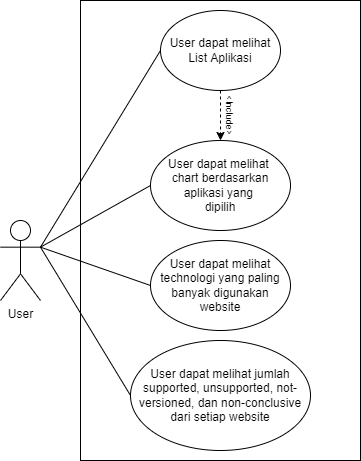
\includegraphics[scale=0.7]{Gambar/usecase.png}  
	\caption{UseCase Diagram} 
	\label{fig:usecase_diagram} 
\end{figure}
Pada aplikasi ini terdapat empat buah aksi, yaitu:
\begin{enumerate}
	\item Pengguna dapat melihat daftar aplikasi.
	\item Setelah daftar aplikasi ditampilkan, pengguna dapat melihat chart berdasarkan aplikasi yang dipilih.
	\item Pengguna dapat melihat tekologi yang paling banyak digunakan \textit{website}.
	\item Pengguna dapat melihat jumlah \textit{supported}, \textit{unsupported}, \textit{not-versioned}, dan \textit{non-conclusive} dari setiap \textit{website}
\end{enumerate}

\subsection{Perancangan Antarmuka}
Antarmuka yang dibuat digunakan untuk mempermudah interaksi antara pengguna dan perangkat lunak yang dapat dilihat pada Gambar \ref{fig:list1}, Gambar \ref{fig:appurl}, dan Gambar \ref{fig:popular}
\begin{figure}[H]
	\centering  
	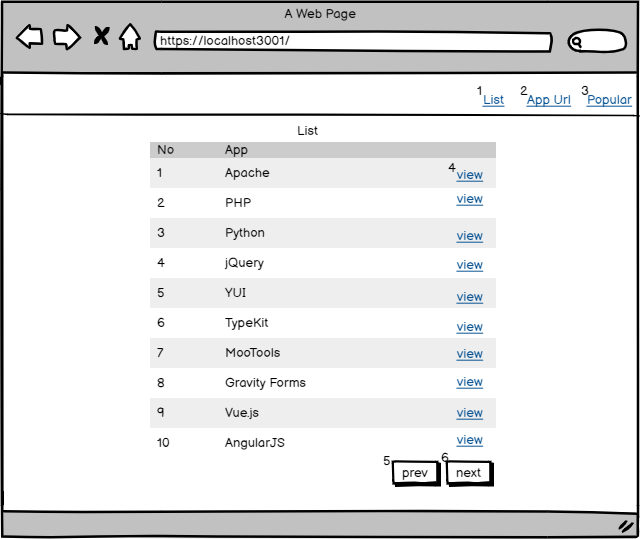
\includegraphics[scale=0.7]{Gambar/list1.png}  
	\caption{Daftar Aplikasi} 
	\label{fig:list1} 
\end{figure}
Berdasarkan rancangan diatas, berikut adalah fungsi dari setiap komponen dalam antarmuka.
\begin{enumerate}
	\item List: berfungsi untuk membuka halaman list aplikasi.
	\item App Url: berfungsi untuk membuka halaman url dengan jumlah aplikasi yang \textit{supported, unsupported, not-versioned, dan non-conclusive}.
	\item Popular: berfungsi untuk membuka halaman aplikasi yang populer.
	\item View: berfungsi untuk melihat \textit{chart} aplikasi tertentu yang dapat dilihat pada Gambar \ref{fig:list2}.
	\item Prev: berfungsi untuk menunjukkan halaman sebelumnya pada tabel.
	\item Next: berfungsi untuk menunjukkan halaman selanjutnya pada tabel. 
\end{enumerate}

\begin{figure}[H]
	\centering  
	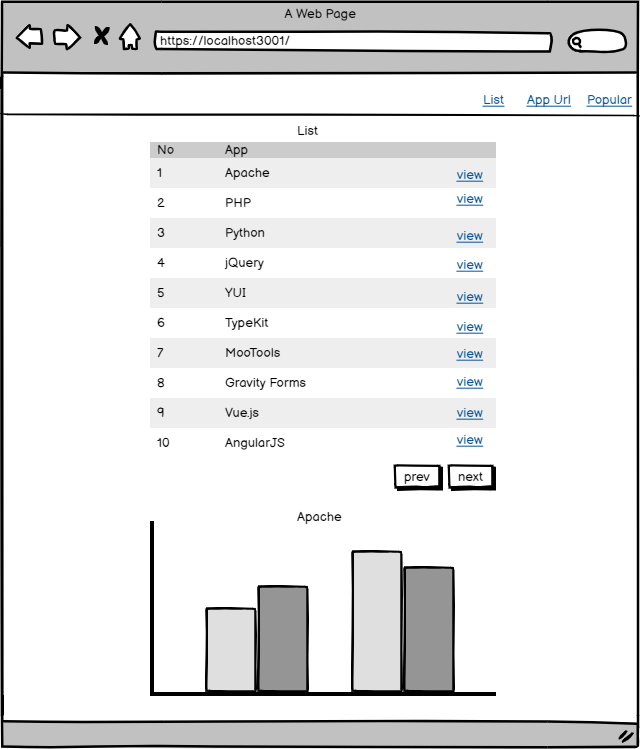
\includegraphics[scale=0.7]{Gambar/list2.png}  
	\caption{Menampilkan Chart Ketika Menekan Tombol View} 
	\label{fig:list2} 
\end{figure}

\begin{figure}[H]
	\centering  
	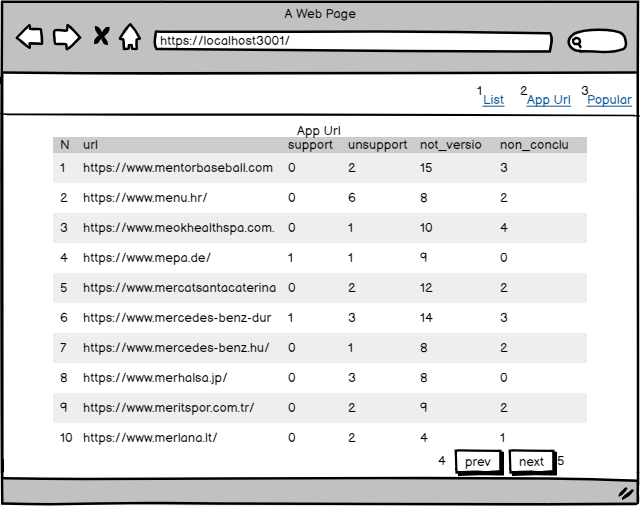
\includegraphics[scale=0.7]{Gambar/appurl.png}  
	\caption{URL dengan Hasil Keseluruhan Aplikasi} 
	\label{fig:appurl} 
\end{figure}
\begin{enumerate}
	\item List: berfungsi untuk membuka halaman list aplikasi.
	\item App Url: berfungsi untuk membuka halaman url dengan jumlah aplikasi yang \textit{supported, unsupported, not-versioned, dan non-conclusive}.
	\item Popular: berfungsi untuk membuka halaman aplikasi yang populer.
	\item Prev: berfungsi untuk menunjukkan halaman sebelumnya pada tabel.
	\item Next: berfungsi untuk menunjukkan halaman selanjutnya pada tabel. 
\end{enumerate}

\begin{figure}[H]
	\centering  
	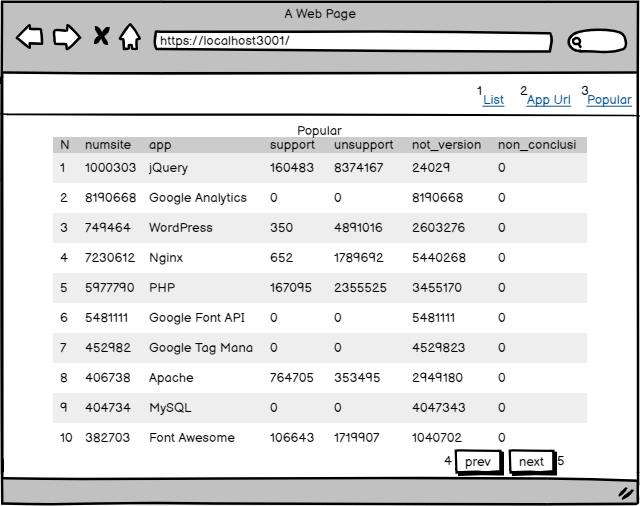
\includegraphics[scale=0.7]{Gambar/popular.png}  
	\caption{Aplikasi yang Populer} 
	\label{fig:popular} 
\end{figure}
\begin{enumerate}
	\item List: berfungsi untuk membuka halaman list aplikasi.
	\item App Url: berfungsi untuk membuka halaman url dengan jumlah aplikasi yang \textit{supported, unsupported, not-versioned, dan non-conclusive}.
	\item Popular: berfungsi untuk membuka halaman aplikasi yang populer.
	\item Prev: berfungsi untuk menunjukkan halaman sebelumnya pada tabel.
	\item Next: berfungsi untuk menunjukkan halaman selanjutnya pada tabel. 
\end{enumerate}

\section{Implementasi Perangkat Lunak}
Perangkat lunak dibuat sesuai dengan data pada Bab \ref{chap:percobaan_awal} dan \ref{chap:penggalian data}. Dalam skripsi ini terdapat tiga bagian yaitu:
\begin{itemize}
	\item BigQuery\\
	Bagian ini adalah representasi dari data. Pada BigQuery dilakukan beberapa \textit{query} untuk mendapatkan data yang diinginkan. Kemudian hasil-hasil dari \textit{query} tersebut disimpan dalam sebuah dataset.
	\item React.js\\
	Bagian ini merupakan bagian tampilan atau web-client. Pada bagian ini bertujuan untuk menampilkan hasil data atau visualisasi data.
	\item Node.js\\
	Bagian ini adalah sebuah penghubung antara data dari Big\textit{query} dan web-client.
\end{itemize}

\subsection{BigQuery}
Bagian ini adalah representasi dari data. Pada BigQuery dilakukan beberapa \textit{query} untuk mendapatkan data yang diinginkan. Kemudian hasil-hasil dari \textit{query} tersebut disimpan dalam sebuah dataset.

\subsubsection{Minimal Supported Data}
Minimal supported data didapatkan dengan mencari sendiri informasi versi dari setiap aplikasi berdasarkan dokumen resminya. Kemudian data-data tersebut dimasukkan kedalam excel dan didownload sebagai csv. Data-data csv tersebut di-upload menggunakan fitur yang ada pada BigQuery dan terbentuk tabel yang berisi csv tersebut. Tabel dari excel tersebut dapat dilihat pada lampiran\ref{lamp:A}

\subsubsection{Menyatukan Tabel Informasi Versi dan Minimal Supported}
\begin{lstlisting}[label={lst:satukan}, caption={Menyatukan Tabel Informasi Versi dan Minimal Supported}]
SELECT 
	jumlah.url, app1.category, app1.app, app1.info, sup.min_supported
FROM(
	SELECT 
		url,  count(app) as jumlah
	FROM
	 	`httparchive.technologies.2020_08_01_*`
	GROUP BY 
		url
	ORDER BY 
		jumlah desc
) AS jumlah

JOIN 

(
	SELECT 
		url, category, app, info
	FROM 
		`httparchive.technologies.2020_08_01_*`
) AS app1
ON jumlah.url = app1.url


JOIN 

(
	SELECT DISTINCT 
		app, min_supported
	FROM 
		`httparchive-bigquery-346414.Step.min_supported_app`
) AS sup
ON app1.app = sup.app

ORDER BY 
	jumlah.jumlah desc
\end{lstlisting}
\textit{Query} pada Gambar \ref{lst:satukan} terdapat beberapa \textit{query} yang disatukan sehingga membentuk suatu tabel yang menyatukan informasi versi yang dipakai aplikasi dengan \textit{minimal supported}.
\begin{itemize}
	\item Mencari url dan jumlah app yang dipakai url tersebut. \textit{Query} yang dilakukan dapat dilihat pada Gambar \ref{lst:satusatu}
	\begin{lstlisting}[label={lst:satusatu}, caption={Mencari URL dan Jumlah APP yang Dipakai}]
SELECT 
	url,  count(app) as jumlah
FROM 
	`httparchive.technologies.2020_08_01_*`
GROUP BY 
	url
ORDER BY 
	jumlah desc
	\end{lstlisting}
	\item Mencari url, kategori, app, informasi versi. \textit{Query} yang dilakukan dapat dilihat pada Gambar \ref{lst:duadua}
	\begin{lstlisting}[label={lst:duadua}, caption={Mencari URL, Kategori, APP, dan Informasi Versi}]
SELECT
	url, category, app, info
FROM 
	`httparchive.technologies.2020_08_01_*`
	\end{lstlisting}
	\item Mencari app dan minimal supported. \textit{Query} yang dilakukan dapat dilihat pada Gambar \ref{lst:tigatiga}
	\begin{lstlisting}[label={lst:tigatiga}, caption={Mencari APP dan Minimal Supported}]
		SELECT DISTINCT
			app, min_supported
		FROM 
			`httparchive-bigquery-346414.Step.min_supported_app`
	\end{lstlisting}
\end{itemize}
\subsubsection{Version Compare}
\begin{lstlisting}[caption={Version Compare Query}, label={lst:versioncomparee}]
CREATE TEMP FUNCTION normaizedSemanticVersion(semanticVersion STRING) 
AS ((
SELECT STRING_AGG(
	IF(isDigit, REPEAT('0', 100 - LENGTH(chars)) || chars, chars) ORDER BY grp 
)
FROM (
	SELECT 
		grp, isDigit, STRING_AGG(char, '' ORDER BY OFFSET) chars,
	FROM (
		SELECT 
			OFFSET, char, isDigit,
			COUNTIF(NOT isDigit) OVER(ORDER BY OFFSET) AS grp
		FROM 
			UNNEST(SPLIT(semanticVersion, '')) AS char WITH OFFSET, 
			UNNEST([char IN ('1','2','3','4','5','6','7','8','9','0')]) isDigit
)
	GROUP BY 
		grp, isDigit
)));
CREATE TEMP FUNCTION compareSemanticVersions(
normSemanticVersion1 STRING, 
normSemanticVersion2 STRING) 
AS ((
SELECT CASE 
WHEN info < min_supported 
	THEN 'UNSUPPORTED'
ELSE 
	'SUPPORTED'
END
FROM 
	UNNEST([STRUCT(
	normaizedSemanticVersion(normSemanticVersion1) AS info, 
	normaizedSemanticVersion(normSemanticVersion2) AS min_supported
)])
));
WITH test AS (
SELECT 
	url, category, app, if (array_length(split(info , ".")) > 2, split(info , ".")[offset(0)] || "." || split(info , ".")[offset(1)], info)  as info, min_supported	
FROM 
	`httparchive-bigquery-346414.app_min_supported_and_info.app_min_supported_and_info`
WHERE 
	info != "\\"
)
SELECT 
	url, category, app, info, min_supported, if(info = '', "NOT VERSIONED",if(min_supported = '?','NON CONCLUSIVE',compareSemanticVersions(info, min_supported)) ) as  result
FROM test 

ORDER BY url
\end{lstlisting}

\textit{Query} pada Gambar \ref{lst:versioncomparee} adalah \textit{query} yang dilakukan untuk melakukan \textit{version compare}. Berikut ini adalah beberapa \textit{step} atau \textit{query} yang dilakukan untuk membuat \textit{version compare} tersebut:
\begin{enumerate}
	\item Normalisasi pada Versi\\
	Pada bagian ini \textit{query} digunakan untuk menormalisasikan digit dari setiap informasi versi sehingga dapat di bandingkan. Berikut ini adalah \textit{query} yang digunakan:
	\begin{itemize}
		\item  Memeriksa Digit Dari Versi. \textit{Query} yang dilakukan dapat dilihat pada Gambar \ref{lst:p}
		\begin{lstlisting}[label={lst:p}, caption={Memeriksa Digit dari Versi}]
SELECT 
	OFFSET, char, isDigit,
	COUNTIF(NOT isDigit) OVER(ORDER BY OFFSET) AS grp
FROM 
	UNNEST(SPLIT('3.14', '')) AS char WITH OFFSET, 
	UNNEST([char IN ('1','2','3','4','5','6','7','8','9','0')]) isDigit
		\end{lstlisting}
		Pada \textit{query} ini mengembalikan \textit{offset} atau \textit{index} yang dimulai dari nol, char sebagai input atau parameter berupa informasi versi, isDigit adalah setiap angka dari setiap input, dan jumlah boolean yang bernilai \textit{false} jika input berupa angka. Hasil dapat dilihat pada Tabel \ref{table:compare_version_step_1}:
		\begin{table}[H]
			\centering
			\begin{tabular}{|l|l|l|l|}
				\hline
				\textbf{OFFSET} & \textbf{char} & \textbf{isDigit} & \textbf{grp}\\
				\hline
				0 & 3 & true & 0\\
				\hline
				1 & . & false & 1\\
				\hline
				2 & 1 & true & 1\\
				\hline
				3 & 4 & true & 1\\
				\hline
			\end{tabular}
			\caption{Hasil Memotong Setiap Char}
			\label{table:compare_version_step_1}
		\end{table}
		
		\item Memotong Setiap Char Dari Version. \textit{Query} dapat dilihat pada Gambar \ref{lst:pp}
		\begin{lstlisting}[label={lst:pp}, caption={Memotong Char dari Setiap Version}]
SELECT 
	grp, isDigit, STRING_AGG(char, '' ORDER BY OFFSET) chars,
FROM (
	SELECT 
		OFFSET, char, isDigit,
		COUNTIF(NOT isDigit) OVER(ORDER BY OFFSET) AS grp
	FROM 
		UNNEST(SPLIT('3.14', '')) AS char WITH OFFSET, 
		UNNEST([char IN ('1','2','3','4','5','6','7','8','9','0')]) isDigit
	)
	GROUP BY grp, isDigit
		\end{lstlisting}
		Pada \textit{query} ini mengembalikan jumlah boolean yang bernilai \textit{false}, \textit{boolean} yang menandakan apakah input merupakan digit atau bukan, dan input yang dibagi-bagi dalam bentuk \textit{string}. Hasil \textit{query} dapat dilihat pada Tabel \ref{table:compare_version_step_2}:

			\begin{table}[H]
			\centering
			\begin{tabular}{|l|l|l|}
				\hline
				\textbf{grp} & \textbf{isDigit} & \textbf{chars}\\
				\hline
				0 & true & 3\\
				\hline
				1 & false & .\\
				\hline
				1 & true & 14\\
				\hline
			\end{tabular}
						\caption{Hasil Memotong Char yang Dipisahkan Titik}
			\label{table:compare_version_step_2}
		\end{table}
		
		\item Normalisasi Informasi Versi. \textit{Query} dapat dilihat pada Gambar \ref{lst:ppp}
		\begin{lstlisting}[label={lst:ppp}, caption={Normalisasi Informasi Versi}]
CREATE TEMP FUNCTION normaizedSemanticVersion(semanticVersion STRING) 
AS ((
SELECT STRING_AGG(
IF(isDigit, REPEAT('0', 100 - LENGTH(chars)) || chars, chars) ORDER BY grp 
)
FROM (
SELECT 
		grp, isDigit, STRING_AGG(char, '' ORDER BY OFFSET) chars,
FROM (
	SELECT 
		OFFSET, char, isDigit,
		COUNTIF(NOT isDigit) OVER(ORDER BY OFFSET) AS grp
	FROM 
	UNNEST(SPLIT(semanticVersion, '')) AS char WITH OFFSET, 
	UNNEST([char IN ('1','2','3','4','5','6','7','8','9','0')]) isDigit
)
GROUP BY 
	grp, isDigit
)));
		\end{lstlisting}
		Pada \textit{query} ini menghasilkan informasi versi yang sudah dinormalisasikan dengan membuat panjang dari setiap versi sama yang dipisahkan oleh isDigit. Pada Tabel \ref{table:compare_version_step_3}, parameter yang digunakan akalah "3.14". Hasil \textit{query} dapat dilihat pada Tabel \ref{table:compare_version_step_3}:
		\begin{table}[H]
			\centering
			\begin{tabular}{|l|p{8cm}|}
				\hline
				\textbf{Row} & \textbf{f0$\_$}\\
				\hline
				1 & 00000000000000000000000000000000000000000 00000000000000000000000000000000000000000 000000000000000003,.,00000000000000000000 00000000000000000000000000000000000000000 000000000000000000000000000000000000014\\
				\hline
			\end{tabular}
						\caption{Hasil Normalisasi Versi}
			\label{table:compare_version_step_3}
		\end{table}
	\end{itemize}

	
	\item Version Compare Function\\
	Pada bagian ini dibuat sebuah fungsi yang digunakan untuk membuat version compare dari informasi versi dari tabel yang sudah dibuat. \textit{Query} dapat dilihat pada Gambar \ref{lst:z}:
	\begin{itemize}
		\item Membuat Fungsi Untuk Membandingkan Versi
		\begin{lstlisting}[label={lst:z}, caption={Fungsi Version Compare}]
CREATE TEMP FUNCTION compareSemanticVersions(
normSemanticVersion1 STRING, 
normSemanticVersion2 STRING) 
AS ((
SELECT CASE 
WHEN info < min_supported 
	THEN 'UNSUPPORTED'
ELSE 
	'SUPPORTED'
END
FROM 
	UNNEST([STRUCT(
	normaizedSemanticVersion(normSemanticVersion1) AS info, 
	normaizedSemanticVersion(normSemanticVersion2) AS min_supported
)])
));
		\end{lstlisting}
		Pada \textit{query} ini menghasilkan UNSUPPORTED jika info atau informasi versi lebih kecil daripada minimal supported yang sudah ditentukan dan mengembalikan SUPPORTED jika info atau informasi versi lebih besar daripada minimal supported yang sudah ditentukan.
	\end{itemize}
		

	\item Membuat Tabel Sementara\\
	Pada bagian ini dibuat sebuah tabel sementara yang beguna membuat group untuk menunjukkan versi yang dihasilkan hanya versi major dan versi minor. \textit{Query} dapat dilihat pada Gambar \ref{lst:zz}
	\begin{lstlisting}[label={lst:zz}, caption={Membuat Tabel Sementara}]
WITH test AS (
SELECT 
	url, category, app, if (array_length(split(info , ".")) > 2, split(info , ".")[offset(0)] || "." || split(info , ".")[offset(1)], info)  as info, min_supported	
FROM
	`httparchive-bigquery-346414.app_min_supported_and_info.app_min_supported_and_info`
WHERE 
	info != "\\"
)
	\end{lstlisting}
	Pada \textit{query} ini membuat tabel sementara yag mengembalikan url, kategori dari aplikasi, aplikasi yang dipakai, informasi versi dari aplikasi, dan minimal supported dari aplikasi yang sudah ditentukan. Pada bagian informasi versi sudah dilakukan group sehingga yang dihasilkan hanya \textit{major} \textit{version} dan \textit{minor version}. 
	
	
	\item Menampilkan Semua Hasil
	Pada bagian ini untuk menampilkan tabel hasil akhir dari \textit{query} yang dilakukan. \textit{Query} dapat dilihat pada Gambar \ref{lst:zzz}
	\begin{lstlisting}[label={lst:zzz}, caption={Menampilkan Semua Hasil}]
SELECT 
	url, category, app, info, min_supported, if(info = '', "NOT VERSIONED",if(min_supported = '?','NON CONCLUSIVE',compareSemanticVersions(info, min_supported)) ) as  result
FROM 
	test 
ORDER BY 
	url
	\end{lstlisting}
Pada \textit{query} ini mengembalikan url, kategori dari aplikasi, aplikasi yang dipakai, informasi versi, \textit{minimal supported}, dan hasil atau result dari \textit{query} yang menunjukkan jika aplikasi tersebut \textit{SUPPORTED} atau \textit{UNSUPPORTED}.
\end{enumerate}
Ketika semua \textit{query} disatukan, berikut adalah 10 contoh hasilnya dapat dilihat pada Tabel \ref{table:result}:

\begin{adjustwidth}{-2.5 cm}{-2.5 cm}\centering\begin{threeparttable}[!htb]
		\begin{tabular}{|p{2cm}|l|l|l|l|l|}
			\hline
			\textbf{url} & \textbf{category} & \textbf{app} & \textbf{info}  & \textbf{min sup}  & \textbf{result}\\
			\hline
			http://0-1.ru/ & Analytics & Yandex.Metrika & & null & NOT VERSIONED\\
			\hline
			http://0-1.ru/ & Web Frameworks & Microsoft ASP.NET
			& & 3.1.20 & NOT VERSIONED\\
			\hline
			http://0-1.ru/ & Video Players & YouTube & & null & NOT VERSIONED\\
			\hline
			http://0-1.ru/ & Web servers & IIS & 6.0 & 8 &  UNSUPPOERTED\\
			\hline
			http://0-1.ru/ & Operating systems & Windows Server & & null & NOT VERSIONED\\
			\hline
			http://0-1.ru/ & Analytics & Liveinternet & & null & NOT VERSIONED\\
			\hline
			http://0-10-10.cocolog-nifty.com/
			& Tag managers & Google Tag Manager
			& & null & NOT VERSIONED\\
			\hline
			http://0-10-10.cocolog-nifty.com/
			& Reverse proxies
			& Nginx & 1.15 & 1.20 & UNSUPPORTED\\
			\hline
			http://0-10-10.cocolog-nifty.com/
			& Web servers & Nginx & 1.15 & 1.20 &  UNSUPPORTED\\
			\hline
			http://0-10-10.cocolog-nifty.com/
			& JavaScript libraries
			& jQuery & 1.11 & 3 & UNSUPPORTED\\
			\hline
		\end{tabular}
%		\caption{Hasil Perbandingan Aplikasi}
		\label{table:result}
\end{threeparttable}\end{adjustwidth}


\subsection{React.js}
Bagian ini merupakan bagian tampilan atau \textit{web-client}. Pada bagian ini bertujuan untuk menampilkan hasil data atau visualisasi data. Terdapat beberapa file dalam perangkat lunak ini, yaitu:
\begin{itemize}
	\item Components\\
	Didalam foler components terdapat beberapa fungsi yaitu:
	\begin{itemize}
		\item AppUrl.js\\
			Pada fungsi ini digunakan untuk membuat tabel yang menampilkan url dengan jumlah dari setiap result (\textit{supported, unsupported, not versioned, dan non conclusive}). Kode dapat dilihat pada Gambar \ref{lst:q}:
			\begin{lstlisting}[label={lst:q}, caption={Membuat Tabel yang Menampilkan URL dengan Jumlah Setiap Result}]
import React, { useEffect, useState } from "react";

const MAX = 10;

export default function AppUrl() {
	const [step, setStep] = useState(0);
	const [data, setData] = useState([]);
	const [isLoading, setIsLoading] = useState(true);
	function getUrlData() {
		setIsLoading(true);
		fetch(`http://localhost:3000/get/app/url?limit=${MAX}&offset=${step}`)
		.then((res) => res.json())
		.then((data) => {
			setData(data);
			setIsLoading(false);
		});
	}
	useEffect(() => {
		getUrlData();
	}, [step]);
	return (
	<div className="container">
	<h2 className="title">App Url</h2>
	{data[0] && (
		<>
		<table className="table">
		<thead>
		<tr>
		<th>No</th>
		{Object.keys(data[0]).map((val) => (
			<th>{val}</th>
			))}
		</tr>
		</thead>
		<tbody>
		{data.map((val, index) => (
			<tr key={index}>
			<td>{index + 1 + MAX * step}</td>
			{Object.values(val).map((val) => (
				<td>{val}</td>
				))}
			</tr>
			))}
		</tbody>
		</table>
		<div className="action">
		<button
		onClick={() => setStep((prev) => prev - 1)}
		disabled={step <= 0 || isLoading}
		>
		Prev
		</button>
		<button
		onClick={() => setStep((prev) => prev + 1)}
		disabled={isLoading}
		>
		Next
		</button>
		</div>
		</>
		)}
	</div>
	);
}

			\end{lstlisting}
		\item List.js\\
			Pada fungsi ini digunakan untuk membuat tabel yang berisi daftar app dan \textit{chart} app yang dipilih. Kode dapat dilihat pada Gambar \ref{lst:qq}:
			\begin{lstlisting}[label={lst:qq}, caption={Membuat Tabel dan Menampilkan Chart Berdasarkan App yang Dipilih}]
import React, { useEffect, useState } from "react";
import { CategoryScale } from "chart.js";
import { Bar } from "react-chartjs-2";
import Chart from "chart.js/auto";

const MAX = 10;

export default function List() {
	const [step, setStep] = useState(0);
	const [data, setData] = useState([]);
	const [isLoading, setIsLoading] = useState(true);
	const [selectedData, setSelectedDate] = useState();
	
	function color(arr) {
		let temp = [];
		for (let i = 0; i < arr.length; i++) {
			const dataType = arr[i].result;
			switch (dataType) {
				case "SUPPORTED":
				temp.push("blue");
				break;
				case "UNSUPPORTED":
				temp.push("red");
				break;
				default:
				temp.push("green");
			}
		}
		return temp;
	}
	useEffect(() => {
		Chart.register(CategoryScale);
	}, []);
	
	function getListData(page) {
		setIsLoading(true);
		fetch(`http://localhost:3000/get/app/type?limit=${MAX}&offset=${page}`)
		.then((res) => res.json())
		.then((data) => {
			setData(data);
			setIsLoading(false);
		});
	}
	
	function getData(name) {
		fetch(`http://localhost:3000/get/app/name/${name}`)
		.then((res) => res.json())
		.then((data) => {
			setSelectedDate({
				name,
				data: {
					labels: data.map((val) => String(val.info)),
					datasets: [
					{
						label: name,
						data: data.map((val) => String(val.jumlah)),
						backgroundColor: color(data),
					},
					],
				},
			});
		});
	}
	
	useEffect(() => {
		getListData(step);
	}, [step]);
	return (
	<div className="container">
	<h2 className="title">List APP</h2>
	{data[0] && (
		<>
		<table className="table table-hover">
		<thead>
		<tr>
		<th className="no">No</th>
		<th>Name</th>
		<th className="action-head"></th>
		</tr>
		</thead>
		<tbody>
		{data.map((val, index) => (
			<tr key={index} onClick={() => getData(val.app)}>
			<th cla>{index + 1 + MAX * step}</th>
			<td>{val.app}</td>
			<td>View</td>
			</tr>
			))}
		</tbody>
		</table>
		<div className="action">
		<button
		onClick={() => setStep((prev) => prev - 1)}
		disabled={step <= 0 || isLoading}
		>
		Prev
		</button>
		<button
		onClick={() => setStep((prev) => prev + 1)}
		disabled={isLoading}
		>
		Next
		</button>
		</div>
		</>
		)}
	
	{selectedData && (
		<div className="selected">
		<h3 className="title">{selectedData.name}</h3>
		<Bar data={selectedData.data} />
		</div>
		)}
	</div>
	);
}
				
			\end{lstlisting}
		\item Popular.js\\
			Pada fungsi ini digunakan untuk membuat tabel yang berisi app yang popular berdasarkan jumlah url yang menggunakan app tersebut. Kode yang digunakan dapat dilihat pada Gambar \ref{lst:qqq}:
			\begin{lstlisting}[label={lst:qqq}, caption={Membuat Tabel App yang Paling Populer}]
import React, { useEffect, useState } from "react";

const MAX = 10;

export default function Popular() {
	const [step, setStep] = useState(0);
	const [data, setData] = useState([]);
	const [isLoading, setIsLoading] = useState(true);
	function getPopularData() {
		setIsLoading(true);
		fetch(`http://localhost:3000/get/app/popular?limit=${MAX}&offset=${step}`)
		.then((res) => res.json())
		.then((data) => {
			setData(data);
			setIsLoading(false);
		});
	}
	useEffect(() => {
		getPopularData();
	}, [step]);
	return (
	<div className="container">
	<h2 className="title">Popular</h2>
	{data[0] && (
		<>
		<table className="table">
		<thead>
		<tr>
		<th>No</th>
		{Object.keys(data[0]).map((val) => (
			<th>{val}</th>
			))}
		</tr>
		</thead>
		<tbody>
		{data.map((val, index) => (
			<tr key={index}>
			<td>{index + 1 + MAX * step}</td>
			{Object.values(val).map((val) => (
				<td>{val}</td>
				))}
			</tr>
			))}
		</tbody>
		</table>
		<div className="action">
		<button
		onClick={() => setStep((prev) => prev - 1)}
		disabled={step <= 0 || isLoading}
		>
		Prev
		</button>
		<button
		onClick={() => setStep((prev) => prev + 1)}
		disabled={isLoading}
		>
		Next
		</button>
		</div>
		</>
		)}
	</div>
	);
}
				
			\end{lstlisting}
		\item Navbar.js\\
			Pada fungsi ini digunakan untuk membuat \textit{header} yang merujuk ke tabel pada AppUrl.js dan tabel pada Popular.js. Kode yang digunakan dapat dilihat pada Gambar \ref{menubar}:
			\begin{lstlisting}[label={lst:menubar}, caption={Membuat menu bar}]
import React from "react";
import { Link } from "react-router-dom";

export default function Navbar() {
	return (
	<ul className="menu">
	<li className="item">
	<a href="/">List</a>
	</li>
	<li className="item">
	<a href="/app-url">App Url</a>
	</li>
	<li className="item">
	<a href="/popular">Popular</a>
	</li>
	</ul>
	);
}
				
			\end{lstlisting}
		
	\end{itemize}
	
	\item App.js\\
	Dalam fungsi ini memanggil components yang dibuat untuk ditampilkan. Kode yang digunakan dapat dilihat pada Gambar \ref{lst:main}:
	\begin{lstlisting}[label={lst:main}, caption={Komponen Utama}]
import * as React from "react";
import Navbar from "./components/Navbar";
import { BrowserRouter, Routes, Route } from "react-router-dom";
import List from "./components/List";
import Popular from "./components/Popular";
import AppUrl from "./components/AppUrl";

function App() {
	return (
	<main className="app">
	<Navbar />
	<BrowserRouter>
	<Routes>
	<Route path="/" element={<List />} />
	<Route path="/app-url" element={<AppUrl />} />
	<Route path="/popular" element={<Popular />} />
	</Routes>
	</BrowserRouter>
	</main>
	);
}

export default App;
	\end{lstlisting}
\end{itemize}

`\subsection{Node.js}
Bagian ini adalah sebuah penghubung antara data dari BigQuery dan web-client. Terdapat tiga bagian utama dalam perangkat lunak yang dibuat yaitu:
\begin{enumerate}
	\item Features\\
	Bagian ini merupakan sebuah folder yang berisi media untuk berkomunikasi dengan BigQuery. Dalam Features terdapat kelas GetApplication.js. Kelas GetApplication.js memiliki beberapa function untuk mendapatkan data dari BigQuery. Kode yang digunakan dapat dilihat pada Gambar \ref{lst:b}:
	\begin{lstlisting}[label={lst:b}, caption={Media untuk Komunikasi dengan BigQuery}]
const {BigQuery} = require('@google-cloud/bigquery');
const options = {
	keyFilename: 'gsm-bigquery-credentials.json',
	projectId: 'httparchive-bigquery-346414',
};
const bigquery = new BigQuery(options)


async function getApplications(app = "Apache") {
	const getAppSql = `select app, info, count(app) as jumlah, result from httparchive-bigquery-346414.app_result.app_result where app = "${app}"  and (result != "NON CONCLUSIVE" and result != "NOT VERSIONED")
	group by app, info, result order by info ASC`
	const options = {
		query: getAppSql,
		location: 'US',
	};
	const [job] = await bigquery.createQueryJob(options);
	const [rows] = await job.getQueryResults();
	return rows.filter(item => !item.info.includes("\\"));
}

async function getApplicationsType(limit = 5 , offset = 1) {
	const getAppSql = `select app from httparchive-bigquery-346414.Step.app_result where info != '' group by app  limit ${limit} offset ${offset}`
	const options = {
		query: getAppSql,
		location: 'US',
	};
	const [job] = await bigquery.createQueryJob(options);
	const [rows] = await job.getQueryResults();
	return rows;
}

async function getApplicationsUrl(limit = 10, offset = 1) {
	const getAppSql = `select * from \`httparchive-bigquery-346414.URL_Result.url_result\` limit ${limit} offset ${offset} `
	
	const options = {
		query: getAppSql,
		location: 'US',
	};
	const [job] = await bigquery.createQueryJob(options);
	const [rows] = await job.getQueryResults();
	return rows;
}

async function getPopularTech(limit = 10, offset = 1) {
	const getAppSql = `select * from \`httparchive-bigquery-346414.numsite_app_result_count.numsite_app_result_count\` limit ${limit} offset ${offset} `
	
	const options = {
		query: getAppSql,
		location: 'US',
	};
	const [job] = await bigquery.createQueryJob(options);
	const [rows] = await job.getQueryResults();
	return rows;
}

module.exports = {getApplications, getApplicationsType, getApplicationsUrl, getPopularTech}
	\end{lstlisting}
	Berikut ini adalah penjelasan setiap fungsi:
	\begin{itemize}
		\item function getApplications(app = "Apache")\\
		Pada fungsi ini mengembalikan app, info, jumlah app, result. Pada fungsi terdapat parameter untuk menentukan app yang ingin ditampilkan. Data tidak menampilkan result yang UNVERSIONED dan NON CONCLUSIVE.
		
		\item function getApplicationType(limit = 5, offset = 1)\\
		Pada fungsi ini mengembalikan semua app. Pada fungsi ini terdapat parameter limit untuk membatasi data dan offset sebagai index data.
		
		\item function getApplicationsUrl(limit = 10, offset = 1)\\
		Pada fungsi ini mengembalikan semua isi tabel. Pada fungsi ini terdapat parameter limit untuk membatasi data dan offset sebagai index data.
		
		\item function getPopularTech(limit = 10, offset = 1)\\
		Pada fungsi ini mengembalikan semua isi tabel. Pada fungsi ini terdapat parameter limit untuk membatasi data dan offset sebagai index data.
		
	\end{itemize}

	\item Router
	Bagian ini berfungsi sebagai penghubung antara backend logic dengan web-client. Kode yang digunakan dapat dilihat pada Gambar \ref{lst:bb}:
	\begin{lstlisting}[label={lst:bb}, caption={Penghubung Backend Logic dengan Web-Client}]
const express = require('express')
const {GetPopularTech} = require("./Controllers/GetPopularTech");
const {GetAppRecap} = require("./Controllers/GetRecap");
const {GetAppType} = require("./Controllers/GetType");
const {GetAppByName} = require("./Controllers/GetApplications");
const cors = require('cors')
const app = express()
const port = 3000
app.use(cors())
app.get('/get/app/name/:name', GetAppByName())
app.get('/get/app/type', GetAppType())
app.get('/get/app/url', GetAppRecap())
app.get('/get/app/popular', GetPopularTech())
app.listen(port, () => {
	console.log(`Listening at http://localhost:${port}`)
})
	\end{lstlisting}
	
	
	\item Controllers
	Bagian ini berfungsi untuk mengimplementasikan \textit{feature} berdasarkan \textit{use-case} yang di berikan.
	Kode yang digunakan dapat dilihat pada Gambar \ref{lst:bbb}:
	\begin{itemize}
		\item GetApplications.js
		\begin{lstlisting}[label={lst:bbb}, caption={Mendapatkan Aplikasi dan Hasilnya}]
const {getApplications} = require("../Features/GetApplications");
const GetAppByName = () => {
	return (req, res) => {
		const {name} = req.params
		getApplications(name).then((rows) => {
			res.send(rows);
		}).catch((e) => {
			res.send(e.message)
		});
	};
}
module.exports = {GetAppByName}
\end{lstlisting}

\item GetPopularTech.js
\begin{lstlisting}[label={lst:bbbb}, caption={Mendapatkan Aplikasi yang Populer}]
const {getPopularTech} = require("../Features/GetApplications");
const GetPopularTech = () => {
	return (req, res) => {
		const {limit, offset} = req.query
		getPopularTech(limit, offset).then((rows) => {
			res.send(rows);
		}).catch((e) => {
			res.send(e.message)
		});
	};
}
module.exports = {GetPopularTech}
\end{lstlisting}

\item GetRecap.js
\begin{lstlisting}[label={lst:bbbbb}, caption={Mendapatkan URL dengan Jumlah Jumlah Result dari Aplikasi}]
const {getApplicationsUrl} = require("../Features/GetApplications");
const GetAppRecap = () => {
	return (req, res) => {
		const {limit, offset} = req.query
		getApplicationsUrl(limit, offset).then((rows) => {
			res.send(rows);
		}).catch((e) => {
			res.send(e.message)
		});
	};
}
module.exports = {GetAppRecap}
\end{lstlisting}

\item GetType.js
\begin{lstlisting}[label={lst:bbbbbb}, caption={Mendapatkan Daftar Apliakasi}]
const {getApplicationsType} = require("../Features/GetApplications");
const GetAppType = () => {
	return (req, res) => {
		const {limit, offset} = req.query
		getApplicationsType(limit , offset).then((rows) => {
			res.send(rows);
		}).catch((e) => {
			res.send(e.message)
		});
	};
}
module.exports = {GetAppType}
		\end{lstlisting}
	
	\end{itemize}
\end{enumerate}

\section{Pengujian Fungsional}
Pada bagian ini, pengujian dilakukan untuk menguji perangkat lunak yang dibangun sudah berjalan dengan sesuai. Terdapat beberapa halaman pada perangkat lunak ini, yaitu:
\subsection{Daftar Aplikasi}
Berikut ini beberapa fitur yang ada pada perangkat lunak:

\begin{enumerate}
	\item Melihat \textit{chart} dari setiap aplikasi.\\
	Fitur ini bertujuan untuk melihat \textit{chart} dari setiap aplikasi yang dipilih yang dapat dilihat pada Gambar \ref{fig:show_chart}
	\begin{figure}[H]
		\centering  
		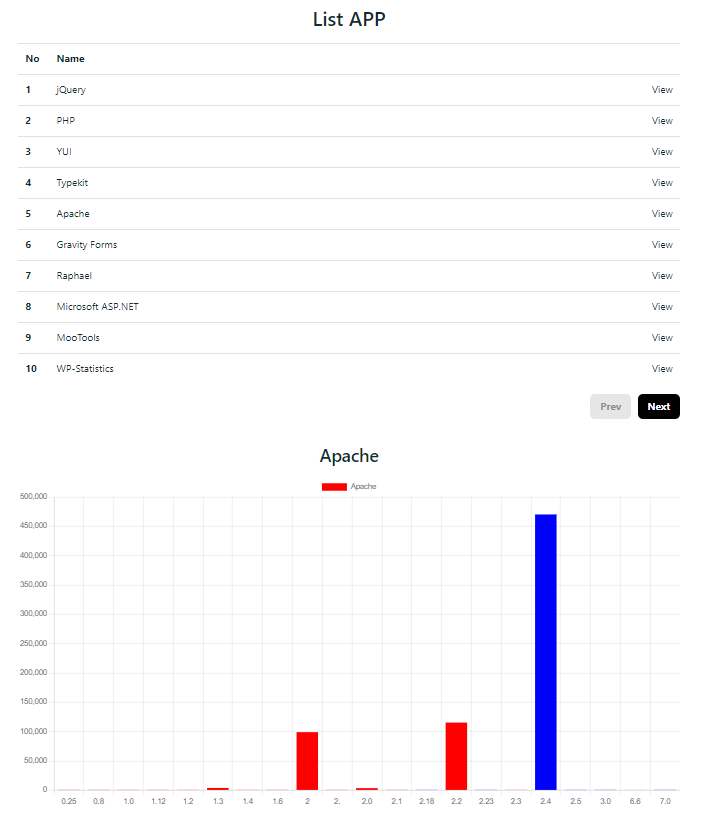
\includegraphics[scale=0.7]{Gambar/pengujian1.png}  
		\caption{Menampilkan \textit{Chart}} 
		\label{fig:show_chart} 
	\end{figure}
	\item Melihat halaman selanjutnya dengan tombol next\\
	Fitur ini bertujuan untuk melihat halaman selanjutnya pada tabel yang dapat dilihat pada Gambar \ref{fig:next}
	\begin{figure}[H]
		\centering  
		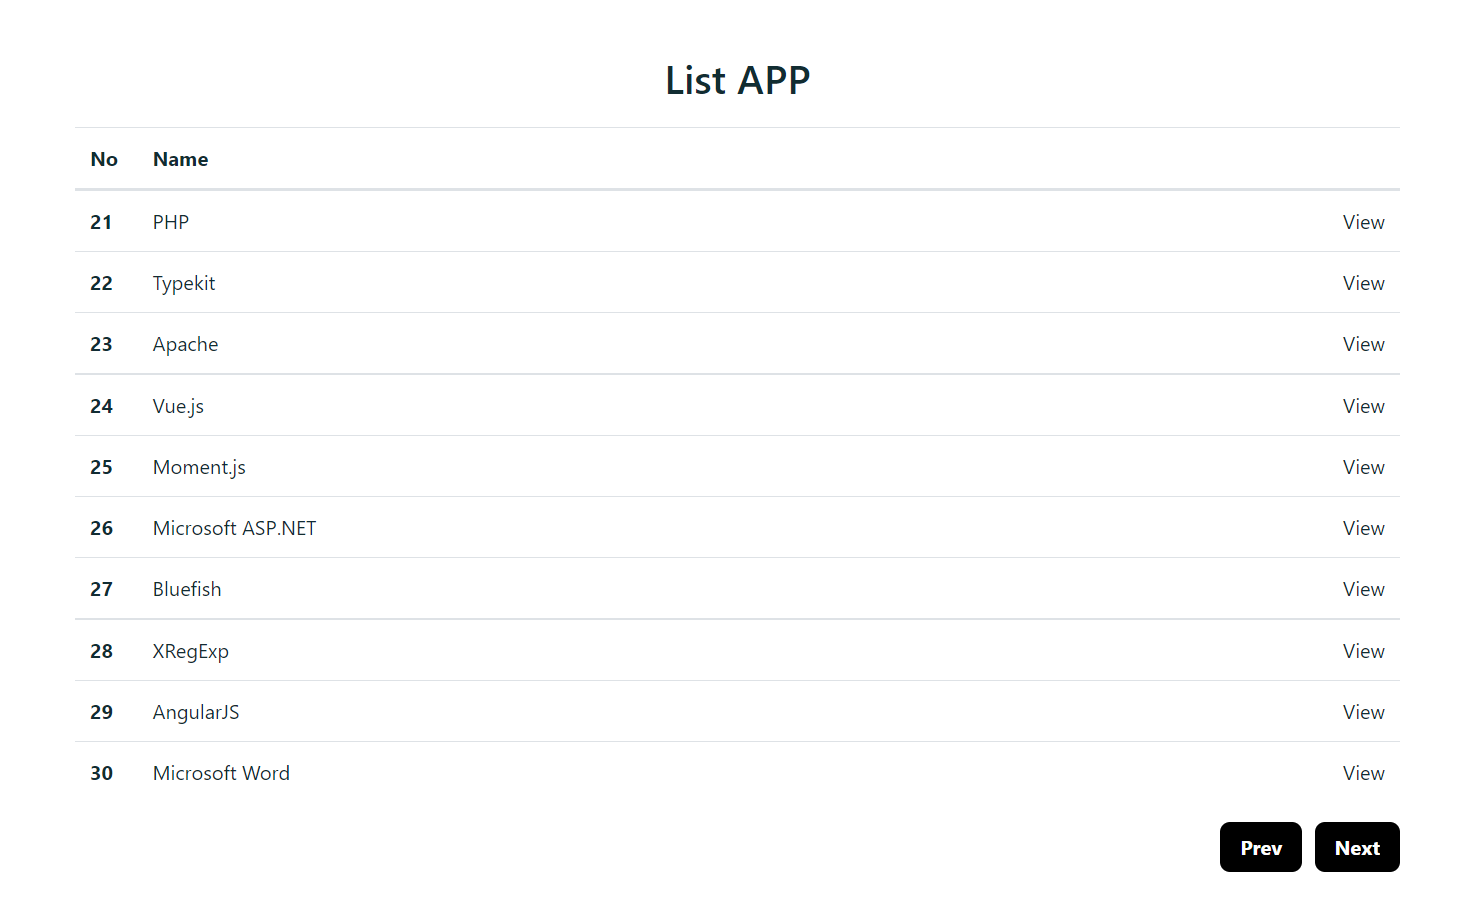
\includegraphics[scale=0.5]{Gambar/pengujian2.png}  
		\caption{Melakukan Tombol Next} 
		\label{fig:next} 
	\end{figure}
	\item Melihat halaman sebelumnya dengan tombol prev\\
	Fitur ini bertujuan untuk melihat halaman sebelumnya pada tabel yang dapat dilihat pada Gambar \ref{fig:prev}
\end{enumerate}
\begin{figure}[H]
	\centering  
	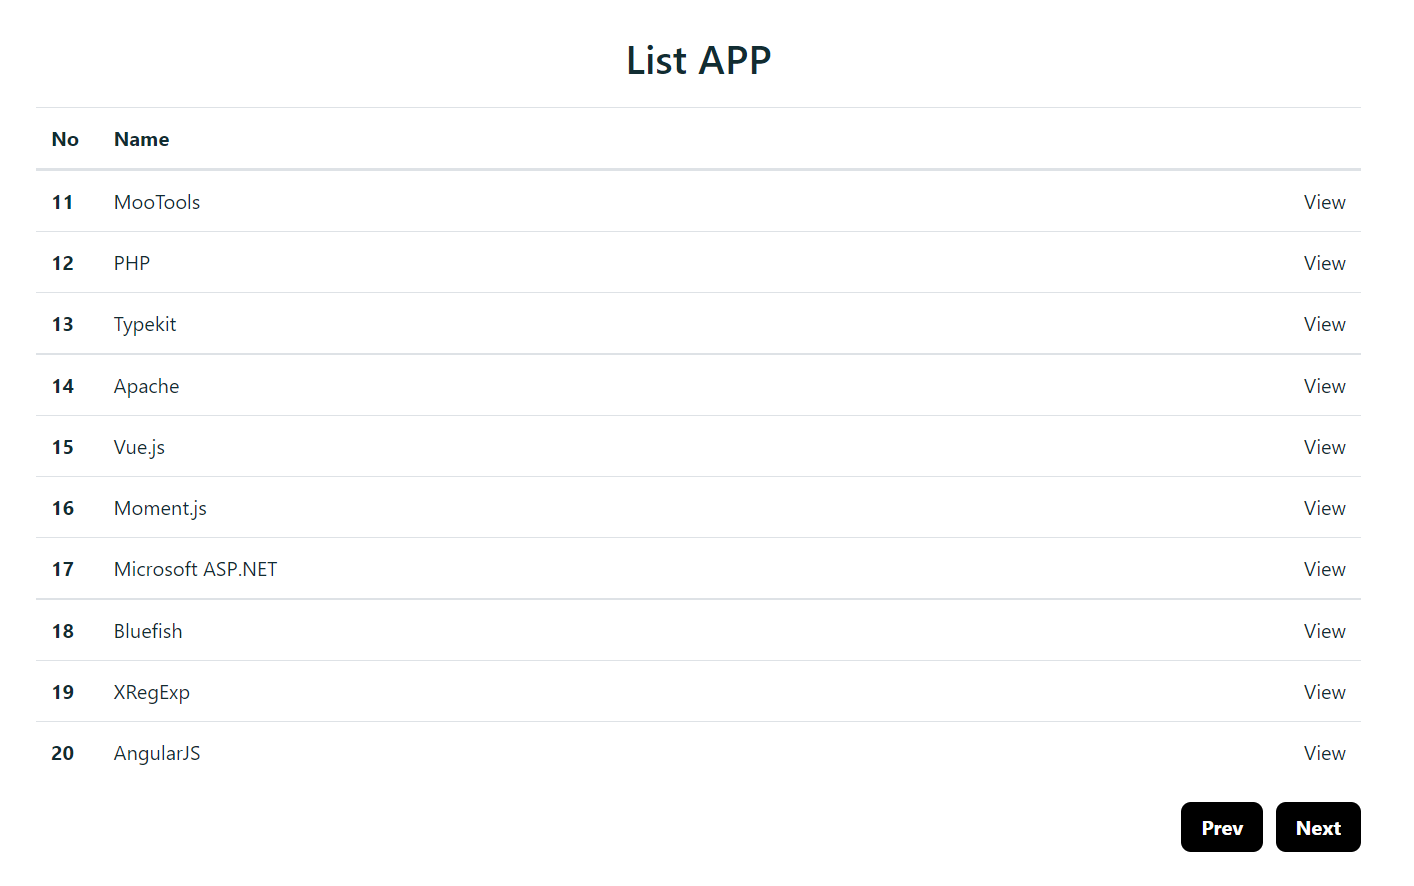
\includegraphics[scale=0.5]{Gambar/pengujian3.png}  
	\caption{Melakukan Tombol Prev} 
	\label{fig:prev} 
\end{figure}


\subsection{Daftar URL dengan Jumlah Hasil Perbandingan}
Berikut ini beberapa fitur yang ada pada perangkat lunak:
\begin{enumerate}
	\item Melihat halaman selanjutnya dengan tombol next\\
	Fitur ini bertujuan untuk melihat halaman selanjutnya pada tabel yang dapat dilihat pada Gambar \ref{fig:app_url_next}
	\begin{figure}[H]
		\centering  
		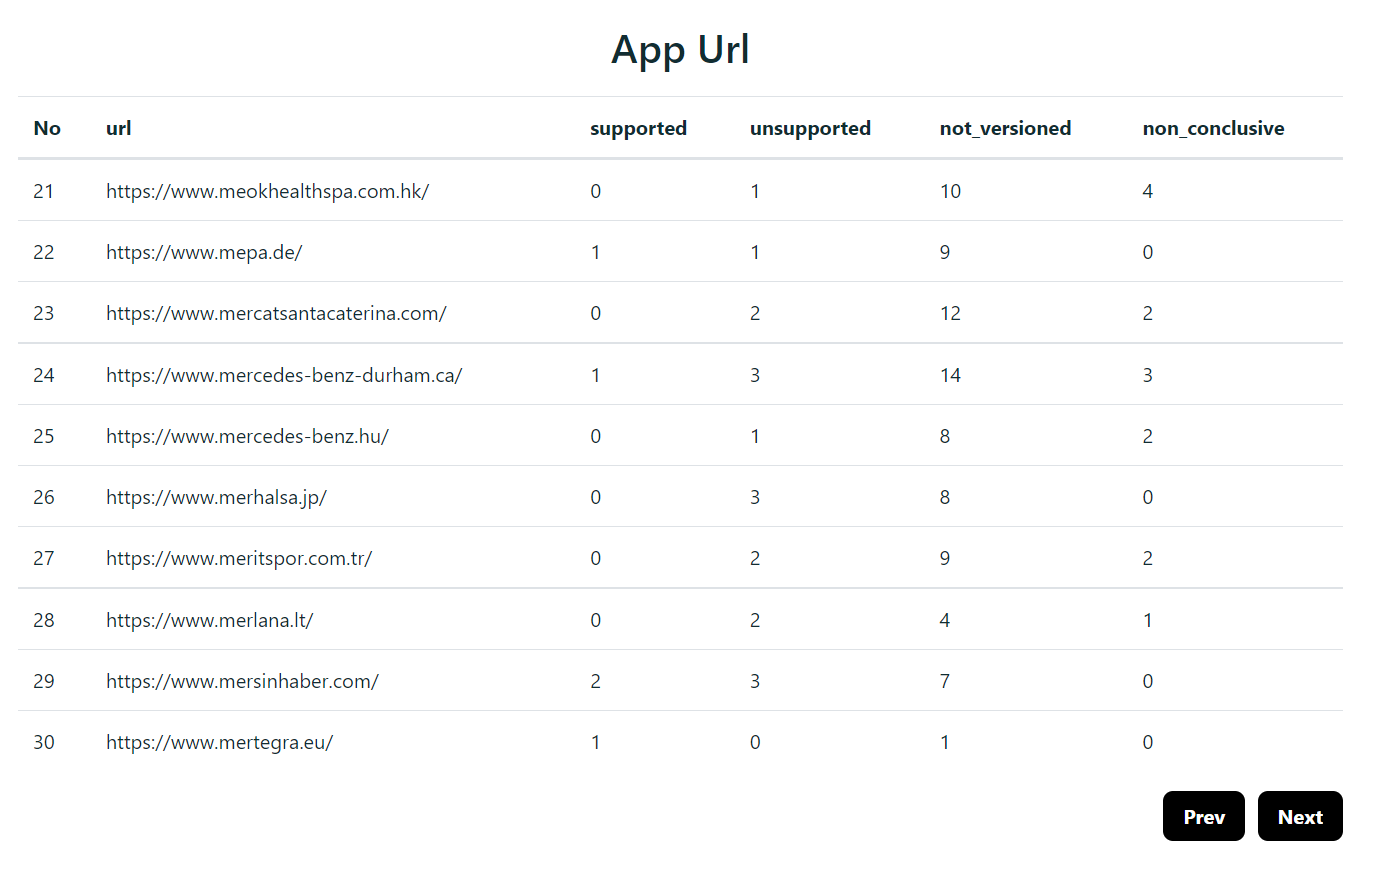
\includegraphics[scale=0.5]{Gambar/pengujian11.png}  
		\caption{Melakukan Tombol Next} 
		\label{fig:app_url_next} 
	\end{figure}
	\item Melihat halaman sebelumnya dengan tombol prev\\
	Fitur ini bertujuan untuk melihat halaman sebelumnya pada tabel yang dapat dilihat pada Gambar \ref{fig:app_url_prev}
\end{enumerate}
\begin{figure}[H]
	\centering  
	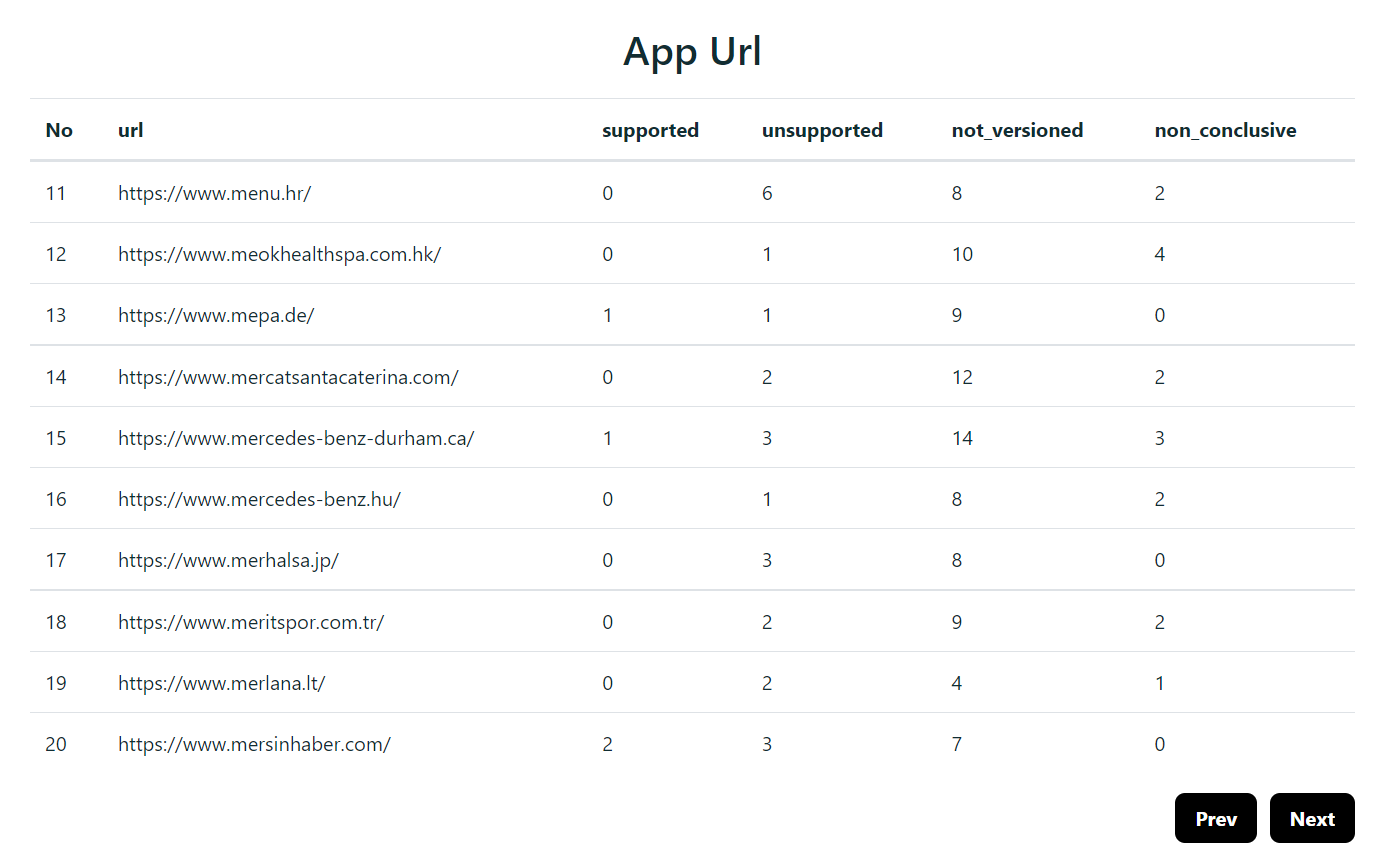
\includegraphics[scale=0.5]{Gambar/pengujian12.png}  
	\caption{Melakukan Tombol Prev} 
	\label{fig:app_url_prev} 
\end{figure}


\subsection{Daftar Aplikasi yang Populer}
Berikut ini beberapa fitur yang ada pada perangkat lunak:
\begin{enumerate}
	\item Melihat halaman selanjutnya dengan tombol next\\
	Fitur ini bertujuan untuk melihat halaman selanjutnya pada tabel yang dapat dilihat pada Gambar \ref{fig:popular_next}
	\begin{figure}[H]
		\centering  
		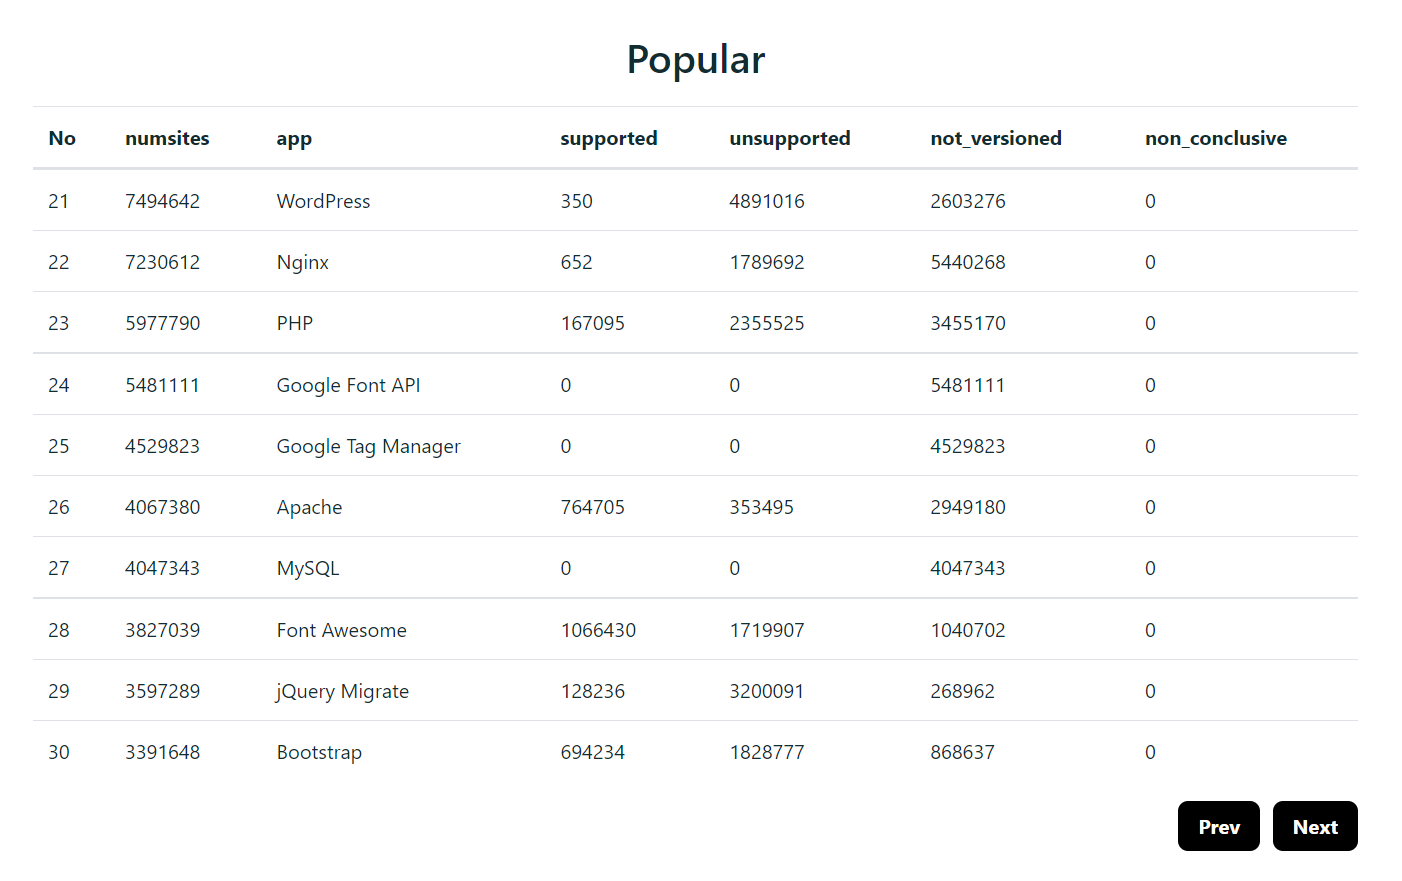
\includegraphics[scale=0.5]{Gambar/pengujian21.png}  
		\caption{Melakukan Tombol Next} 
		\label{fig:popular_next} 
	\end{figure}
	\item Melihat halaman sebelumnya dengan tombol prev\\
	Fitur ini bertujuan untuk melihat halaman sebelumnya pada tabel yang dapat dilihat pada Gambar \ref{fig:popular_prev}
\end{enumerate}
\begin{figure}[H]
	\centering  
	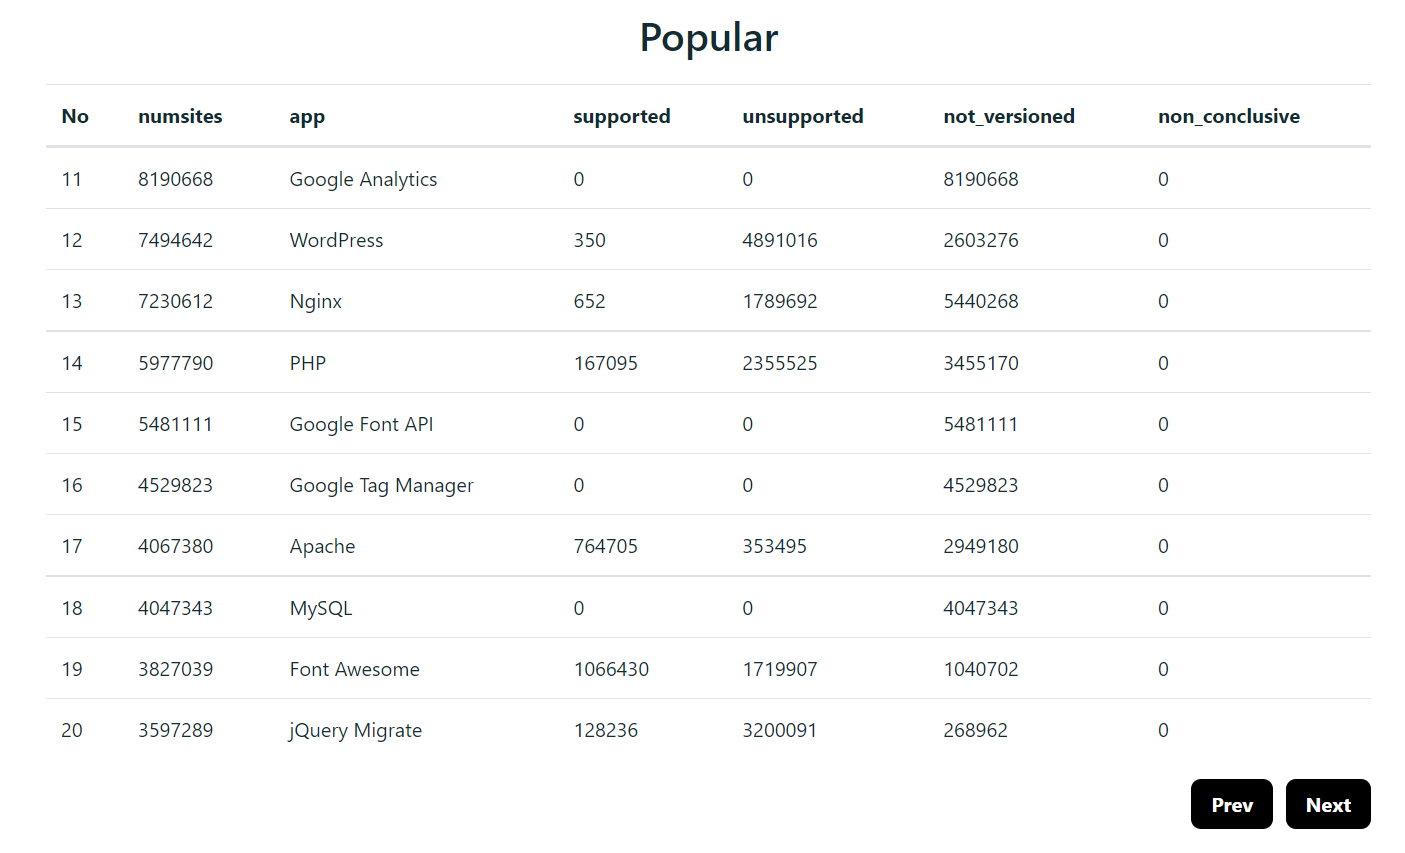
\includegraphics[scale=0.5]{Gambar/pengujian22.png}  
	\caption{Melakukan Tombol Prev} 
	\label{fig:popular_prev} 
\end{figure}